\section{Numerical experiments}
\label{sec:num_exp}

Before we present the proof of our main result, we illustrate our theoretical findings with some numerical examples confirming the rates and the $\kappa$-dependence in our error bounds. In the following we will hence compute discrete minimizers
$$
\solh = \underset{\testfunh \in \VSh}{\mbox{arg\hspace{2pt}min}}\hspace{1pt}\energy(\testfunh) 
$$
in $\mathcal{P}_1$-spaces $\VSh$ for different mesh sizes $h$ and different material parameters $\kappa$. Note that, just like analytical minimizers, discrete minimizers can be at most unique up to gauge transformations, i.e., if $\solh \in \VSh$ is a minimizer, so is $\exp(-\ci \theta) \solh$ for any $\theta \in [-\pi,\pi)$. 


\subsection{Implementation}

For the discretization in space with linear Lagrange finite elements, we use the open source Python tool FEniCS \cite[version 2018.1.0]{Fenics}. 
%
 To compute a discrete minimizer, we applied a steepest descent approach
using an implicit Euler method for the $L^2$ gradient flow. 
A direct application yields the following nonlinear iteration
%
\begin{align}
	\ipsymLtwo{\solh^{n+1}}{ \testfunh } = \ipsymLtwo{\solh^{n}}{ \testfunh } - \tau \, \dualp{\energy'(\solh^{n+1})}{\testfunh} ,
\end{align}
%
where $\tau>0$ is some parameter. To avoid the solution of nonlinear systems several times, we replace $\energy'(u^{n+1})$ by the linearization
%
\begin{align}
	\dualp{\energy'(\solh^{n+1})}{\testfunh} \to  \abilmag{\solh^{n+1}}{\testfunh} + \kappa^2 \Real \int_\Omega (|\solh^{n}|^2 - 1) \solh^{n+1} \testfunh^* \,dx,
\end{align}
%
and thus have to solve the following linear system for $\solh^{n+1} \in \VSh$
%
\begin{align}
	\ipsymLtwo{\solh^{n+1}}{ \testfunh } 
	+ 
	\tau \, \abilmag{\solh^{n+1}}{\testfunh} 
	+
	 \tau \, \kappa^2 \Real \int_\Omega (|\solh^{n}|^2 - 1) \solh^{n+1} \testfunh^* \,dx
	  = 
	  \ipsymLtwo{\solh^{n}}{ \testfunh }
\end{align}
for all $\testfunh \in \VSh$.
%
In our experiments, we  set $\Omega = [0,1] \times [0,1] \subset \R^2$,
and use 
on the finest grid the initial value $\sol_0 = 0.8 + 0.6 \ci$. For the coarser grids, we project this reference solution and use this as a starting value.
%
The magnetic potential is chosen as
%
\begin{equation}
	\MagF(x,y) :=  \sqrt{2} \begin{pmatrix}
		\sin(\pi x) \cos(\pi y) \\ -  \cos(\pi x) \sin(\pi y)
	\end{pmatrix} , 
\end{equation}
%
and satisfies the assumptions in \eqref{eq:ass_\MagF_for_H2}.
%
Further, we set $\tau = \kappa^{-2}$, and used the stopping criterion
%
$ \kappa^{-2} | \energy(\solh^{n+1}) - \energy(\solh^{n})| < \delta $
for a tolerance $\delta = 10^{-9}$. Below this tolerance, we use a Newton method for the equation $\energy^{\prime}(\solh)=0$ with the previous approximation $\solh^{n}$ as starting value and the same stopping criterion, but $\delta = 10^{-12}$.
%
The code to reproduce the results presented in this paper is available at \url{\mycode}.

Let us note that the steepest descent approach as described above can potentially also find local minimizers of $\energy$ in $\VSh$, depending on the choice of the initial value. However, we also note that global minimizers are typically found more easily and that local minimizers (that are not global minimizers) can be identified and discarded by comparing the energy levels. 

Finally, let us also mention that the phase of the minimizer (i.e. which $\exp(- \ci \theta) u_h$ we find for some $\theta \in [-\pi,\pi)$) depends only on the choice of the initial value. Hence, it is important to start the steepest descent method always with the same initial value in order to ensure a reasonable comparison between minimizers on different meshes (since phase differences might otherwise dominate the error).

\subsection{Numerical results}

We first illustrate the convergence in the spatial parameter $\h$ for different values of $\kappa$.
To this end, we computed a reference solution on a finer grid using $\h_{\text{max}} \sim  2.5 \cdot 10^{-3}$. %0.00248592 
%
In order to numerically verify Assumption~\ref{ass:cinfsup} on the local uniqueness of the computed minimizers, we proceeded as in Remark~\ref{rem:loc_uniq} and computed the $5$ smallest eigenvalues (in absolute value) of $\energy''$ and collected them in Table~\ref{tab:eigs_L2}.
We observe that the first eigenvalue is essentially zero up to numerical precision and we verified that it indeed belongs to $\ci \solh$. The second smallest eigenvalue is clearly bounded away from zero, and the computed minimum is hence indeed locally unique in the sense of Definition~\ref{def-local-uniqueness}.
%
\begin{table}
	\begin{center}
		\begin{tabular}{ |c|c|c|c|c|c| } 
			\hline
			$\kappa$ & 		$\lambda_1 $ &	$\lambda_2 $ &	$\lambda_3 $ &	$\lambda_4 $ &	$\lambda_5 $  \\
			\hline
			$8$ & \Zeile{1.70e-14 }{ 4.15e-02 }{ 4.15e-02 }{ 1.18e-01 }{ 1.20e-01 } \\ 
			\hline
			$ 10$	& \Zeile{2.86e-14 }{ 3.37e-02 }{ 3.37e-02 }{ 3.78e-02 }{ 1.07e-01}\\ 
			\hline
			$ 17$	& \Zeile{3.93e-11 }{ 1.59e-03 }{ 1.99e-03 }{ 9.12e-03 }{ 9.50e-03 } \\ 
			\hline
			$ 24$	& \Zeile{1.19e-12 }{ 8.94e-04 }{ 3.52e-03 }{ 3.52e-03 }{ 9.59e-03 } \\ 
			\hline
		\end{tabular}
	\end{center}
	\caption{
		The numerically computed $5$ smallest eigenvalues of $\energy''(\solh)$ with reference solution $\solh$ and $\kappa = 8,10,17,24$.}
	\label{tab:eigs_L2}
\end{table}



In order to compare the results for different values of $\kappa$, we divide the error in the $\HonekappaSpace$- and $L^2$-norm by $\kappa^2$
and the energy by $\kappa^4$, see Figure~\ref{fig:convergence}. Here we recall that according to Corollary~\ref{cor:main_Lagrange} we expect the $\HonekappaSpace$-error to convergence with the rate $\kappa^2 \h$, the $L^2$-error with the rate $\kappa^2 \h^2$ and the energy-error with the rate $\kappa^4 \h^2$. 
%
Indeed, we observe the predicted asymptotic convergence in $\h$ and, in particular, the numerical experiments confirm the $\kappa$-scaling in our error estimates. The plot further indicates that the constants in front of the normalized errors are independent of $\kappa$.
Further, we observe in Figure~\ref{fig:uniformness} the uniform boundedness of $\Honekappa{\solh}$ and $\energy(\solh)$ as predicted in Lemma~\ref{lem:bound_general_uH}.



\begin{figure}
	\centering
     \begin{subfigure}{0.45\textwidth}
  			\resizebox{1.0\textwidth}{!}{% This file was created by tikzplotlib v0.9.8.
\begin{tikzpicture}

%\definecolor{color0}{rgb}{0.12156862745098,0.466666666666667,0.705882352941177}
%\definecolor{color1}{rgb}{1,0.498039215686275,0.0549019607843137}
%\definecolor{color2}{rgb}{0.172549019607843,0.627450980392157,0.172549019607843}
%\definecolor{color3}{rgb}{0.83921568627451,0.152941176470588,0.156862745098039}
%\definecolor{color4}{rgb}{0.580392156862745,0.403921568627451,0.741176470588235}
%\definecolor{color5}{rgb}{0.549019607843137,0.337254901960784,0.294117647058824}
%\definecolor{color6}{rgb}{0.890196078431372,0.466666666666667,0.76078431372549}

\begin{axis}[
legend cell align={left},
legend style={
  fill opacity=0.8,
  draw opacity=1,
  text opacity=1,
  at={(0.03,0.97)},
  anchor=north west,
  draw=white!80!black,
  /tikz/every even column/.append style={column sep=3mm}
},
log basis x={10},
log basis y={10},
tick align=outside,
tick pos=left,
title={\Large$\kappa^{-2}$-weighted $H^1_\kappa$-error},
x grid style={white!69.0196078431373!black},
xmin=0.00405395301108757, xmax=0.361336322303478,
xmode=log,
xtick style={color=black},
y grid style={white!69.0196078431373!black},
ymin=0.00034704390290097, ymax=0.133787233845049,
ymode=log,
ytick style={color=black},
legend columns=-1,
legend to name=Legendforall,
]
\addplot [semithick, color0, mark=asterisk, mark size=3, mark options={solid}]
table {%
0.294627825494395 0.186292767898167
0.158363330156169 0.0487731680809855
0.0791364521303744 0.0209109126023387
0.0397638752183648 0.00998202529110857
0.0198857667264535 0.00470219036719555
0.00994323397220818 0.00217541620918486
0.00497183342869752 0.000984157784530789
};
\addlegendentry{$\kappa  = 8$}
\addplot [semithick, color1, mark=asterisk, mark size=3, mark options={solid}]
table {%
0.294627825494395 0.111342718120629
0.158363330156169 0.0439356983225817
0.0791364521303744 0.0315920990793495
0.0397638752183648 0.0280339645519302
0.0198857667264535 0.00298379934272898
0.00994323397220818 0.00137823159327496
0.00497183342869752 0.000622679540854472
};
\addlegendentry{$\kappa  = 12$}
\addplot [semithick, color2, mark=asterisk, mark size=3, mark options={solid}]
table {%
0.294627825494395 0.0608149420474765
0.158363330156169 0.0649914184458722
0.0791364521303744 0.0629398325948987
0.0397638752183648 0.0684369116888249
0.0198857667264535 0.0709140956934424
0.00994323397220818 0.00206054145256177
0.00497183342869752 0.000890024426947719
};
\addlegendentry{$\kappa  = 24$}
\addplot [semithick, gray, dashed]
table {%
0.294627825494395 0.0527423062958883
0.158363330156169 0.0283491460832591
0.0791364521303744 0.0141664793215857
0.0397638752183648 0.00711826346598202
0.0198857667264535 0.00355981719600055
0.00994323397220818 0.00177997136167936
0.00497183342869752 0.000890024426947719
};
%\addlegendentry{O(h)}
\end{axis}
\end{tikzpicture}
}	
%    		\caption{Error}
     	\end{subfigure}
     \hfill
          \begin{subfigure}{0.45\textwidth}
      \resizebox{1.0\textwidth}{!}{% This file was created by tikzplotlib v0.9.8.
\begin{tikzpicture}

%\definecolor{color0}{rgb}{0.12156862745098,0.466666666666667,0.705882352941177}
%\definecolor{color1}{rgb}{1,0.498039215686275,0.0549019607843137}
%\definecolor{color2}{rgb}{0.172549019607843,0.627450980392157,0.172549019607843}
%\definecolor{color3}{rgb}{0.83921568627451,0.152941176470588,0.156862745098039}
%\definecolor{color4}{rgb}{0.580392156862745,0.403921568627451,0.741176470588235}
%\definecolor{color5}{rgb}{0.549019607843137,0.337254901960784,0.294117647058824}
%\definecolor{color6}{rgb}{0.890196078431372,0.466666666666667,0.76078431372549}

\begin{axis}[
legend cell align={left},
legend style={
  fill opacity=0.8,
  draw opacity=1,
  text opacity=1,
  at={(0.03,0.97)},
  anchor=north west,
  draw=white!80!black
},
log basis x={10},
log basis y={10},
tick align=outside,
tick pos=left,
title={\Large$\kappa^{-2}$-weighted $L^2$-error},
x grid style={white!69.0196078431373!black},
xmin=0.00405395301108757, xmax=0.361336322303478,
xmode=log,
xtick style={color=black},
y grid style={white!69.0196078431373!black},
ymin=6.32426386908231e-07, ymax=0.0158602697316919,
ymode=log,
ytick style={color=black}
]
\addplot [semithick, color0, mark=asterisk, mark size=3, mark options={solid}]
table {%
	0.294627825494395 0.0230599035621619
	0.158363330156169 0.00368818487123406
	0.0791364521303744 0.000858103337433082
	0.0397638752183648 0.000223078179724807
	0.0198857667264535 5.50295921136434e-05
	0.00994323397220818 1.30880277376933e-05
	0.00497183342869752 2.75631372947969e-06
};
\addlegendentry{kappa = 8}
\addplot [semithick, color1, mark=asterisk, mark size=3, mark options={solid}]
table {%
	0.294627825494395 0.0103844137646045
	0.158363330156169 0.00358790831455995
	0.0791364521303744 0.00284351477136656
	0.0397638752183648 0.00266986515680828
	0.0198857667264535 3.03845029941999e-05
	0.00994323397220818 7.24826900759356e-06
	0.00497183342869752 1.56385327985216e-06
};
\addlegendentry{kappa = 12}
\addplot [semithick, color2, mark=asterisk, mark size=3, mark options={solid}]
table {%
	0.294627825494395 0.00261864223939326
	0.158363330156169 0.00280855035174448
	0.0791364521303744 0.00255182358218369
	0.0397638752183648 0.00275763245532324
	0.0198857667264535 0.0028350257122837
	0.00994323397220818 2.86177090176729e-05
	0.00497183342869752 5.64433667715548e-06
};
\addlegendentry{kappa = 24}
\addplot [semithick, gray, dashed]
table {%
	0.294627825494395 0.0198210789670603
	0.158363330156169 0.00572649680029844
	0.0791364521303744 0.00142998974416575
	0.0397638752183648 0.000361041542028175
	0.0198857667264535 9.02951558488044e-05
	0.00994323397220818 2.25753809979132e-05
	0.00497183342869752 5.64433667715548e-06
};
\legend{}
\end{axis}

\end{tikzpicture}
}	
%     	% This file was created by tikzplotlib v0.9.8.
\begin{tikzpicture}

%\definecolor{color0}{rgb}{0.12156862745098,0.466666666666667,0.705882352941177}
%\definecolor{color1}{rgb}{1,0.498039215686275,0.0549019607843137}
%\definecolor{color2}{rgb}{0.172549019607843,0.627450980392157,0.172549019607843}
%\definecolor{color3}{rgb}{0.83921568627451,0.152941176470588,0.156862745098039}
%\definecolor{color4}{rgb}{0.580392156862745,0.403921568627451,0.741176470588235}
%\definecolor{color5}{rgb}{0.549019607843137,0.337254901960784,0.294117647058824}
%\definecolor{color6}{rgb}{0.890196078431372,0.466666666666667,0.76078431372549}

\begin{axis}[
legend cell align={left},
legend style={
  fill opacity=0.8,
  draw opacity=1,
  text opacity=1,
  at={(0.03,0.97)},
  anchor=north west,
  draw=white!80!black
},
log basis x={10},
log basis y={10},
tick align=outside,
tick pos=left,
title={\Large$\kappa^{-2}$-weighted $L^2$-error},
x grid style={white!69.0196078431373!black},
xmin=0.00405395301108757, xmax=0.361336322303478,
xmode=log,
xtick style={color=black},
y grid style={white!69.0196078431373!black},
ymin=6.32426386908231e-07, ymax=0.0158602697316919,
ymode=log,
ytick style={color=black}
]
\addplot [semithick, color0, mark=asterisk, mark size=3, mark options={solid}]
table {%
	0.294627825494395 0.0230599035621619
	0.158363330156169 0.00368818487123406
	0.0791364521303744 0.000858103337433082
	0.0397638752183648 0.000223078179724807
	0.0198857667264535 5.50295921136434e-05
	0.00994323397220818 1.30880277376933e-05
	0.00497183342869752 2.75631372947969e-06
};
\addlegendentry{kappa = 8}
\addplot [semithick, color1, mark=asterisk, mark size=3, mark options={solid}]
table {%
	0.294627825494395 0.0103844137646045
	0.158363330156169 0.00358790831455995
	0.0791364521303744 0.00284351477136656
	0.0397638752183648 0.00266986515680828
	0.0198857667264535 3.03845029941999e-05
	0.00994323397220818 7.24826900759356e-06
	0.00497183342869752 1.56385327985216e-06
};
\addlegendentry{kappa = 12}
\addplot [semithick, color2, mark=asterisk, mark size=3, mark options={solid}]
table {%
	0.294627825494395 0.00261864223939326
	0.158363330156169 0.00280855035174448
	0.0791364521303744 0.00255182358218369
	0.0397638752183648 0.00275763245532324
	0.0198857667264535 0.0028350257122837
	0.00994323397220818 2.86177090176729e-05
	0.00497183342869752 5.64433667715548e-06
};
\addlegendentry{kappa = 24}
\addplot [semithick, gray, dashed]
table {%
	0.294627825494395 0.0198210789670603
	0.158363330156169 0.00572649680029844
	0.0791364521303744 0.00142998974416575
	0.0397638752183648 0.000361041542028175
	0.0198857667264535 9.02951558488044e-05
	0.00994323397220818 2.25753809979132e-05
	0.00497183342869752 5.64433667715548e-06
};
\legend{}
\end{axis}

\end{tikzpicture}

%     	\caption{Error}
     \end{subfigure}
 \hfill
      \begin{subfigure}{0.45\textwidth}
    \resizebox{1.0\textwidth}{!}{% This file was created by tikzplotlib v0.9.8.
\begin{tikzpicture}

%\definecolor{color0}{rgb}{0.12156862745098,0.466666666666667,0.705882352941177}
%\definecolor{color1}{rgb}{1,0.498039215686275,0.0549019607843137}
%\definecolor{color2}{rgb}{0.172549019607843,0.627450980392157,0.172549019607843}
%\definecolor{color3}{rgb}{0.83921568627451,0.152941176470588,0.156862745098039}
%\definecolor{color4}{rgb}{0.580392156862745,0.403921568627451,0.741176470588235}
%\definecolor{color5}{rgb}{0.549019607843137,0.337254901960784,0.294117647058824}
%\definecolor{color6}{rgb}{0.890196078431372,0.466666666666667,0.76078431372549}

\begin{axis}[
legend cell align={left},
legend style={
  fill opacity=0.8,
  draw opacity=1,
  text opacity=1,
  at={(0.03,0.97)},
  anchor=north west,
  draw=white!80!black
},
log basis x={10},
log basis y={10},
tick align=outside,
tick pos=left,
title={\Large $\kappa^{-4}$-weighted energy-error},
x grid style={white!69.0196078431373!black},
ymin=1.5784742274581e-07, ymax=0.0026678922926463,
xmode=log,
xtick style={color=black},
y grid style={white!69.0196078431373!black},
ymin=1.5784742274581e-07, ymax=0.0026678922926463,
ymode=log,
ytick style={color=black}
]
\addplot [semithick, color0, mark=asterisk, mark size=3, mark options={solid}]
table {%
0.294627825494395 0.000720846857710871
0.158363330156169 0.000692078225095722
0.0791364521303744 0.000198378428186978
0.0397638752183648 5.25609342789976e-05
0.0198857667264535 1.30001997395855e-05
0.00994323397220818 3.07387671049254e-06
0.00497183342869752 6.13243152043641e-07
};
\addlegendentry{kappa = 8}
\addplot [semithick, color1, mark=asterisk, mark size=3, mark options={solid}]
table {%
0.294627825494395 0.00060805108156661
0.158363330156169 0.000264072384994007
0.0791364521303744 7.18516808995838e-05
0.0397638752183648 1.512966760044e-05
0.0198857667264535 5.21843865227579e-06
0.00994323397220818 1.23365010869988e-06
0.00497183342869752 2.45706229756283e-07
};
\addlegendentry{kappa = 12}
\addplot [semithick, color2, mark=asterisk, mark size=3, mark options={solid}]
table {%
0.294627825494395 0.000235808147364608
0.158363330156169 0.000165385263624264
0.0791364521303744 8.27030322592656e-05
0.0397638752183648 4.04121587736161e-05
0.0198857667264535 2.72448888091635e-05
0.00994323397220818 2.42409324224933e-06
0.00497183342869752 4.88062273899721e-07
};
\addlegendentry{kappa = 24}
\addplot [semithick, gray, dashed]
table {%
0.294627825494395 0.00171391634219181
0.158363330156169 0.000495166608530809
0.0791364521303744 0.000123650321749152
0.0397638752183648 3.12190370726319e-05
0.0198857667264535 7.80776583793484e-06
0.00994323397220818 1.95207912181929e-06
0.00497183342869752 4.88062273899721e-07
};
%\addlegendentry{O(h**2)}
\legend{}
\end{axis}

\end{tikzpicture}
}
% 	% This file was created by tikzplotlib v0.9.8.
\begin{tikzpicture}

%\definecolor{color0}{rgb}{0.12156862745098,0.466666666666667,0.705882352941177}
%\definecolor{color1}{rgb}{1,0.498039215686275,0.0549019607843137}
%\definecolor{color2}{rgb}{0.172549019607843,0.627450980392157,0.172549019607843}
%\definecolor{color3}{rgb}{0.83921568627451,0.152941176470588,0.156862745098039}
%\definecolor{color4}{rgb}{0.580392156862745,0.403921568627451,0.741176470588235}
%\definecolor{color5}{rgb}{0.549019607843137,0.337254901960784,0.294117647058824}
%\definecolor{color6}{rgb}{0.890196078431372,0.466666666666667,0.76078431372549}

\begin{axis}[
legend cell align={left},
legend style={
  fill opacity=0.8,
  draw opacity=1,
  text opacity=1,
  at={(0.03,0.97)},
  anchor=north west,
  draw=white!80!black
},
log basis x={10},
log basis y={10},
tick align=outside,
tick pos=left,
title={\Large $\kappa^{-4}$-weighted energy-error},
x grid style={white!69.0196078431373!black},
ymin=1.5784742274581e-07, ymax=0.0026678922926463,
xmode=log,
xtick style={color=black},
y grid style={white!69.0196078431373!black},
ymin=1.5784742274581e-07, ymax=0.0026678922926463,
ymode=log,
ytick style={color=black}
]
\addplot [semithick, color0, mark=asterisk, mark size=3, mark options={solid}]
table {%
0.294627825494395 0.000720846857710871
0.158363330156169 0.000692078225095722
0.0791364521303744 0.000198378428186978
0.0397638752183648 5.25609342789976e-05
0.0198857667264535 1.30001997395855e-05
0.00994323397220818 3.07387671049254e-06
0.00497183342869752 6.13243152043641e-07
};
\addlegendentry{kappa = 8}
\addplot [semithick, color1, mark=asterisk, mark size=3, mark options={solid}]
table {%
0.294627825494395 0.00060805108156661
0.158363330156169 0.000264072384994007
0.0791364521303744 7.18516808995838e-05
0.0397638752183648 1.512966760044e-05
0.0198857667264535 5.21843865227579e-06
0.00994323397220818 1.23365010869988e-06
0.00497183342869752 2.45706229756283e-07
};
\addlegendentry{kappa = 12}
\addplot [semithick, color2, mark=asterisk, mark size=3, mark options={solid}]
table {%
0.294627825494395 0.000235808147364608
0.158363330156169 0.000165385263624264
0.0791364521303744 8.27030322592656e-05
0.0397638752183648 4.04121587736161e-05
0.0198857667264535 2.72448888091635e-05
0.00994323397220818 2.42409324224933e-06
0.00497183342869752 4.88062273899721e-07
};
\addlegendentry{kappa = 24}
\addplot [semithick, gray, dashed]
table {%
0.294627825494395 0.00171391634219181
0.158363330156169 0.000495166608530809
0.0791364521303744 0.000123650321749152
0.0397638752183648 3.12190370726319e-05
0.0198857667264535 7.80776583793484e-06
0.00994323397220818 1.95207912181929e-06
0.00497183342869752 4.88062273899721e-07
};
%\addlegendentry{O(h**2)}
\legend{}
\end{axis}

\end{tikzpicture}

% 	\caption{Error}
 \end{subfigure}
 \hfill
 \begin{subfigure}{0.45\textwidth}
 %\vspace{-21mm}
  %\hspace{8mm}
  \resizebox{0.85\textwidth}{!}{\begin{centering}\ref{Legendforall}\end{centering}}\\[4.0em]
\end{subfigure}
%
%\ref{Legendforall}
%
\caption{Convergence in the mesh size $\h$ for $\kappa$-weighted errors
	in the $\HonekappaSpace$- and $L^2$-norm and for the energy,
	for $\kappa = 8,10,17,24$. The errors between $\sol$ and $\solh$ in $L^2$ and $\HonekappaSpace$ are scaled by $\kappa^{-2}$ and the error in energy by $\kappa^{-4}$. The dotted lines indicate the corresponding errors (in $L^2$ and $\HonekappaSpace$ respectively) between $\sol$ and its best-approximation $\textup{R}_{\kappa,\h}(u)$ in $\VSh$ with respect to 
	$\abilmagstabsym{\cdot}{\cdot}$, cf. \eqref{best-approxi-H1kappa}.
	The dashed lines indicate order $\mathcal{O}(\h)$ in the upper left figure, and 
	order $\mathcal{O}(\h^2)$ in the upper left and bottom right figure.
}
\label{fig:convergence}
\end{figure}




\begin{figure}
	\centering
	\begin{subfigure}{0.45\textwidth}
		\resizebox{1.0\textwidth}{!}{% This file was created by tikzplotlib v0.9.8.
\begin{tikzpicture}


\begin{axis}[
legend cell align={left},
legend style={
  fill opacity=0.8,
  draw opacity=1,
  text opacity=1,
  at={(0.03,0.97)},
  anchor=north west,
  draw=white!80!black,
  /tikz/every even column/.append style={column sep=3mm}
},
log basis x={10},
log basis y={10},
tick align=outside,
tick pos=left,
title={\large$\kappa^{-1}$-weighted $H^1_\kappa$-norm},
x grid style={white!69.0196078431373!black},
xmin=0.004, xmax=0.5,
xmode=log,
xtick style={color=black},
y grid style={white!69.0196078431373!black},
ymin=0.1, ymax=1.2,
%ymode=log,
ytick style={color=black},
legend columns=4,
%legend to name=Legendforall,
xlabel style={font=\color{white!15!black}},
xlabel={maximal mesh width $h$},
]
\addplot [semithick, color0, mark=asterisk, mark size=3, mark options={solid}]
table {%
0.294627825494395 0.514401168043143
0.158363330156169 0.811869089884772
0.0791364521303744 0.913859595264147
0.0397638752183648 0.939726535166265
0.0198857667264535 0.946574925856512
0.00994323397220818 0.948278890596904
0.00497183342869752 0.948700283533424
};
%\addlegendentry{$\kappa  = 8$}
\addplot [semithick, color1, mark=asterisk, mark size=3, mark options={solid}]
table {%
0.294627825494395 0.417479625304531
0.158363330156169 0.745380738833216
0.0791364521303744 0.824444492260676
0.0397638752183648 0.845729527170419
0.0198857667264535 0.851446858467175
0.00994323397220818 0.852866879728289
0.00497183342869752 0.853217652795658
};
%\addlegendentry{$\kappa  = 10$}
\addplot [semithick, color3, mark=asterisk, mark size=3, mark options={solid}]
table {%
0.294627825494395 0.362387981191403
0.158363330156169 0.56133771645226
0.0791364521303744 0.835631639361613
0.0397638752183648 0.910916062611938
0.0198857667264535 0.932330453552667
0.00994323397220818 0.93767568616111
0.00497183342869752 0.938995366743317
};
%\addlegendentry{$\kappa  = 17$}
\addplot [semithick, color2, mark=asterisk, mark size=3, mark options={solid}]
table {%
0.294627825494395 0.24921514809579
0.158363330156169 0.477769520000272
0.0791364521303744 0.667854785983945
0.0397638752183648 0.907515286403963
0.0198857667264535 0.951484305324516
0.00994323397220818 0.963023480356877
0.00497183342869752 0.965860492400518
};
%\addlegendentry{$\kappa  = 24$}
\legend{}
\end{axis}
\end{tikzpicture}
}	
		%    		\caption{Error}
	\end{subfigure}
	\hfill
	\begin{subfigure}{0.45\textwidth}
		\resizebox{1.0\textwidth}{!}{% This file was created by tikzplotlib v0.9.8.
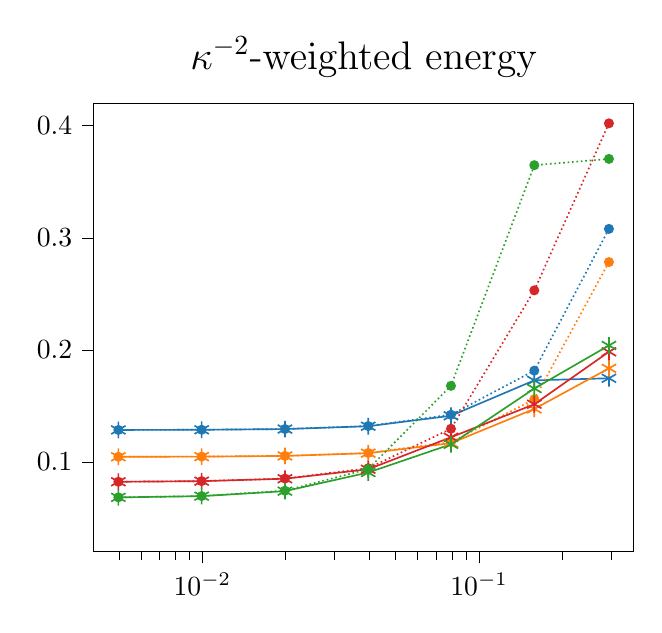
\begin{tikzpicture}

\definecolor{color0}{rgb}{0.12156862745098,0.466666666666667,0.705882352941177}
\definecolor{color1}{rgb}{1,0.498039215686275,0.0549019607843137}
\definecolor{color2}{rgb}{0.172549019607843,0.627450980392157,0.172549019607843}
\definecolor{color3}{rgb}{0.83921568627451,0.152941176470588,0.156862745098039}
\definecolor{color4}{rgb}{0.580392156862745,0.403921568627451,0.741176470588235}
\definecolor{color5}{rgb}{0.549019607843137,0.337254901960784,0.294117647058824}

\begin{axis}[
legend cell align={left},
legend style={
	fill opacity=0.8,
	draw opacity=1,
	text opacity=1,
	at={(0.03,0.97)},
	anchor=north west,
	draw=white!80!black
},
log basis x={10},
%log basis y={10},
tick align=outside,
tick pos=left,
title={\Large$\kappa^{-2}$-weighted energy},
x grid style={white!69.0196078431373!black},
xmin=0.00405395301108757, xmax=0.361336322303478,
xmode=log,
xtick style={color=black},
y grid style={white!69.0196078431373!black},
ymin=0.02, ymax=0.42,
%ymode=log,
ytick style={color=black}
%legend columns=4,
%legend to name=Legendforall,
]
\addplot [semithick, color0, mark=asterisk, mark size=3, mark options={solid}]
table {%
	0.294627825494395 0.174667913751863
	0.158363330156169 0.172826740593055
	0.0791364521303744 0.141229940348444
	0.0397638752183648 0.131897618858136
	0.0198857667264535 0.129365728466913
	0.00994323397220818 0.128730441320605
	0.00497183342869752 0.128572959889447
};
\addlegendentry{ $\kappa = 8$}
\addplot [semithick, color0,densely dotted, mark=*, mark size=1.5, mark options={solid}]
table {%
	0.294627825494395 0.307966533955576
	0.158363330156169 0.181520946333042
	0.0791364521303744 0.142167624331016
	0.0397638752183648 0.132072576409203
	0.0198857667264535 0.129401709133532
	0.00994323397220818 0.128739490297263
	0.00497183342869752 0.12857498871627
};
\addlegendentry{$ \kappa = 8$}
\addplot [semithick, color1, mark=asterisk, mark size=3, mark options={solid}]
table {%
	0.294627825494395 0.183535574986566
	0.158363330156169 0.147347502350145
	0.0791364521303744 0.116776315726729
	0.0397638752183648 0.107846487959398
	0.0198857667264535 0.105404505908502
	0.00994323397220818 0.104792642612376
	0.00497183342869752 0.104640955127579
};
\addlegendentry{$\kappa = 10$}
\addplot [semithick, color1,densely dotted, mark=*, mark size=1.5, mark options={solid}]
table {%
	0.294627825494395 0.278357444397727
	0.158363330156169 0.155981999381869
	0.0791364521303744 0.117693477658881
	0.0397638752183648 0.108018426813211
	0.0198857667264535 0.105439128196237
	0.00994323397220818 0.104801464613601
	0.00497183342869752 0.104642912856309
};
\addlegendentry{$\kappa = 10$}
\addplot [semithick, color3, mark=asterisk, mark size=3, mark options={solid}]
table {%
	0.294627825494395 0.198316077382189
	0.158363330156169 0.151527938494597
	0.0791364521303744 0.122042022471181
	0.0397638752183648 0.0934736833921267
	0.0198857667264535 0.0850577472209076
	0.00994323397220818 0.0828915702964943
	0.00497183342869752 0.0823529985915896
};
\addlegendentry{$\kappa = 17$}
\addplot [semithick, color3,densely dotted, mark=*, mark size=1.5, mark options={solid}]
table {%
	0.294627825494395 0.402158437117071
	0.158363330156169 0.253118243401632
	0.0791364521303744 0.129651541602237
	0.0397638752183648 0.0944299008404986
	0.0198857667264535 0.0852049327704375
	0.00994323397220818 0.0829237392079835
	0.00497183342869752 0.082360029996195
};
\addlegendentry{$\kappa = 17$}
\addplot [semithick, color2, mark=asterisk, mark size=3, mark options={solid}]
table {%
	0.294627825494395 0.203950290466262
	0.158363330156169 0.16554239234541
	0.0791364521303744 0.115761830127568
	0.0397638752183648 0.090583263647513
	0.0198857667264535 0.0739775247394644
	0.00994323397220818 0.0695210460539965
	0.00497183342869752 0.0684059135528233
};
\addlegendentry{$\kappa = 24$}
\addplot [semithick, color2,densely dotted, mark=*, mark size=1.5, mark options={solid}]
table {%
	0.294627825494395 0.370387964660919
	0.158363330156169 0.364801903252744
	0.0791364521303744 0.167934721210636
	0.0397638752183648 0.0936497756663386
	0.0198857667264535 0.0743624619664625
	0.00994323397220818 0.0695916363316121
	0.00497183342869752 0.0684206422077068
};
\addlegendentry{$\kappa = 24$}
\legend{}
\end{axis}

\end{tikzpicture}
}	
	\end{subfigure}
\ref{Legendforall}
%
\caption{Boundedness of the scaled $\HonekappaSpace$-norm and energy $\energy$ with respect to $\h$ for $\kappa = 8,10,17,24$.
		The dotted lines show the energy of the best-approximation $\textup{R}_{\kappa,\h}(u)$ in $\VSh$
		with respect to $\abilmagstabsym{\cdot}{\cdot}$.
%
}
\label{fig:uniformness}
\end{figure}



Let us also note that for larger values of $\kappa$, we observe a preasymptotic behavior in $\h$. We expect that this is related to the smallness condition for $\kappa \Csol \h$ stated in the theorem, which is required below in Lemma~\ref{lem:du_F_inf_sup_solvability_discrete} for the discrete inf-sup stability. Since beyond the (numerically observed) threshold $\kappa h < 1$, the errors coincide for all values of $\kappa$, this is still in alignment with our theory. 
 

To further investigate the preasymptotic effect, we added a comparison of our errors with the 
 	best-approximation $\textup{R}_{\kappa,\h}(u)$ in $\VSh$ with respect to 
 $\abilmagstabsym{\cdot}{\cdot}$. To be precise, for our reference solution $\sol$, we computed the orthogonal projection $\textup{R}_{\kappa,\h}(u) \in \VSh$ such that
 \begin{align}
 \label{best-approxi-H1kappa}
 \abilmagstabsym{\sol  - \textup{R}_{\kappa,\h}(\sol)}{\phi_h} = 0, \quad \text{for all} \quad \phi_h \in \VSh .
 \end{align}
%
By comparing our errors $\Honekappa{ u - u_h}$ with $\Honekappa{ u - \textup{R}_{\kappa,\h}(u) }$, we can identify possible numerical pollution effects related to $\kappa$. The corresponding results are depicted in Figure \ref{fig:convergence} and reveal a very interesting phenomenon. Contrary to $\solh$ itself, the best-approximation does not show any visible preasymptotic convergence. On the contrary, in the asymptotic regime both approximations have a very similar behavior and follow the expected rates closely. Since both errors are expected to behave asymptotically as
\begin{align}
\Honekappa{ \sol - \solh} + \Honekappa{ \sol - \textup{R}_{\kappa,\h}(\sol) } \lesssim \kappa \min \{ 1 , \h \kappa \} 
\end{align}
(due to the energy bounds $\Honekappa{\sol}+\Honekappa{\solh}\lesssim \kappa$), we suspect that the necessary resolution condition $\h \kappa \lesssim 1$ will only become visible for larger values of $\kappa$, whereas the preasymptotic convergence of $\solh$ must be related to the smallness condition $\kappa \Csol \h$. This is further supported by the right-hand side of Figure~\ref{fig:uniformness}, where we compare the energy $\energy(\,\textup{R}_{\kappa,\h}(u) \,)$ of the best-approximation with the energy $\energy(\solh)$ of the actual minimizer in $\VSh$. We can see that, in the preasymptotic regime, the energy of $\textup{R}_{\kappa,\h}(u)$ is indeed significantly larger than the one of $\solh$. This explains why good approximations are not found on coarse meshes and indicates that one cannot capture the correct vortex pattern on meshes which do not satisfy some further resolution condition on $\h$ with respect to $\kappa$.

In our second experiment, we first computed for $\kappa = 20$
the discrete minimizers for different values of 
$h \approx 8\cdot 10^{-2}, 4\cdot 10^{-2}, 2\cdot 10^{-2}, 1 \cdot 10^{-2} $ ,
see Figure~\ref{fig:diff_solutions_in_h}.
%
We observe that the number of vortices remains constant on the different discretization levels, but 
the minimizer is rotated by $\frac{\pi}{2}$. A simple calculation show that by our choice of $\MagF$ this rotation of the coordinate system leaves the energy invariant. In particular, this illustrates that the density $|u|^2$ of minimizers is not necessarily unique and that convergence of discrete minimizers can only be expected up to a subsequence, even for a fixed gauge condition.
%
On the other hand, we plotted the minimizers for the values $\kappa=8,10,17,24$, see Figure~\ref{fig:diff_solutions}.
%
We observe that the number of vortices increases with larger values of $\kappa$, which is in agreement with analytical results \cite{Aftalion99,SaS07}.

\begin{figure}[t!]
	\centering
	\begin{subfigure}{0.2\textwidth}
%		\includegraphics[width=1.4\textwidth]{tikz/plasma/plot_sol_kappa_20_h3.png}	
		\includegraphics[width=1.4\textwidth]{plot_sol_kappa_20_h3.png}		
%		\includegraphics[width=1.4\textwidth]{tikz/red_blue/plot_sol_kappa_20_h3.png}	
	\end{subfigure}
	\hfill
	\begin{subfigure}{0.2\textwidth}
%		\includegraphics[width=1.4\textwidth]{tikz/plasma/plot_sol_kappa_20_h4.png}	
		\includegraphics[width=1.4\textwidth]{plot_sol_kappa_20_h4.png}	
%		\includegraphics[width=1.4\textwidth]{tikz/red_blue/plot_sol_kappa_20_h4.png}
	\end{subfigure}
	\hfill
	\begin{subfigure}{0.2\textwidth}
%		\includegraphics[width=1.4\textwidth]{tikz/plasma/plot_sol_kappa_20_h5.png}	
		\includegraphics[width=1.4\textwidth]{plot_sol_kappa_20_h5.png}	
%		\includegraphics[width=1.4\textwidth]{tikz/red_blue/plot_sol_kappa_20_h5.png}	
	\end{subfigure}
	\hfill
	\begin{subfigure}{0.2\textwidth}
%		\includegraphics[width=1.4\textwidth]{tikz/plasma/plot_sol_kappa_20_h6.png}
		\includegraphics[width=1.4\textwidth]{plot_sol_kappa_20_h6.png}
%		\includegraphics[width=1.4\textwidth]{tikz/red_blue/plot_sol_kappa_20_h6.png}
	\end{subfigure}

	\caption{Minimizers for the Ginzburg--Landau parameter $\kappa =20$ and different mesh widths 
		$h \approx 8\cdot 10^{-2}, 4\cdot 10^{-2}, 2\cdot 10^{-2}, 1 \cdot 10^{-2} $ 
		(from left to right).}
	\label{fig:diff_solutions_in_h}
\end{figure}



\begin{figure}[t!]
	\centering
	\begin{subfigure}{0.2\textwidth}
%		\includegraphics[width=1.4\textwidth]{tikz/plasma/plot_sol_kappa_8_h8.png}	
		\includegraphics[width=1.4\textwidth]{plot_sol_kappa_8_h8.png}	
%		\includegraphics[width=1.4\textwidth]{tikz/red_blue/plot_sol_kappa_8_h8.png}	
	\end{subfigure}
	\hfill
	\begin{subfigure}{0.2\textwidth}
%		\includegraphics[width=1.4\textwidth]{tikz/plasma/plot_sol_kappa_10_h8.png}		
		\includegraphics[width=1.4\textwidth]{plot_sol_kappa_10_h8.png}	
%		\includegraphics[width=1.4\textwidth]{tikz/red_blue/plot_sol_kappa_10_h8.png}	
	\end{subfigure}
	\hfill
	\begin{subfigure}{0.2\textwidth}
%		\includegraphics[width=1.4\textwidth]{tikz/plasma/plot_sol_kappa_17_h8.png}	
		\includegraphics[width=1.4\textwidth]{plot_sol_kappa_17_h8.png}	
%		\includegraphics[width=1.4\textwidth]{tikz/red_blue/plot_sol_kappa_17_h8.png}		
	\end{subfigure}
	\hfill
	\begin{subfigure}{0.2\textwidth}
%		\includegraphics[width=1.4\textwidth]{tikz/plasma/plot_sol_kappa_24_h8.png}
		\includegraphics[width=1.4\textwidth]{plot_sol_kappa_24_h8.png}
%		\includegraphics[width=1.4\textwidth]{tikz/red_blue/plot_sol_kappa_24_h8.png}
	\end{subfigure}
	\caption{Different minimizers corresponding to the Ginzburg--Landau parameters $\kappa = 8,10,17,24$ (from left to right) for $\h \approx 2.5 \cdot 10^{-3}$.
	}
	\label{fig:diff_solutions}
\end{figure}

